\chapter{Technical Background and Disambiguation}
\label{cha:Disambiguation}
% [TODO] General info, introduction of chapter

\section{Intelligent Transportation Systems (ITS)}
Intelligent Transportation Systems (ITS) apply information and communication technologies to vehicles, transportation infrastructure and its users aiming to provide services to enhance road safety, mobility and traffic efficiency. % goals

% .... 


% ...ITS not only for road vehicles
Initially ITS have been only apparent in the road transport domain, yet began to appear in other domains such as in maritime and rail transport. % proof?
This development lead to expansion of ITS original ``Fundamental services'' which have been defined in the international standard ISO 141813-1 in 1999. % citation
With the most recent version (2016), ITS are now expected to address the following service domains:

% service domains (where each holds different service groups)
\begin{multicols}{2}
    \begin{itemize}
        \item Traveler information
        \item Traffic management\\and operations
        \item Vehicle services
        \item Freight transport
        \item Public transport
        \item Emergency
        \columnbreak
        \item Transport-related electronic\\payment
        \item Road transport-related\\personal safety
        \item Weather and environmental\\conditions monitoring
        \item Disaster response management\\and coordination
        \item National security.
    \end{itemize}
\end{multicols}

While ITS offer services to different domains, generally ITS services are about enhancing the driving experience. ITS can exist without intercommunication with other ITS or other vehicles, such as \textit{lane departure warning systems} and \textit{adaptive cruise control} that use technologies like video pattern recognition and radar to provide assistance to the driver. \cite{} % Intelligent Transport Systems Standards by Bob Williams

However, \textbf{Cooperative Intelligent Transportation Systems} (C-ITS) are the most promising technology to contribute to ``improving road safety by avoiding accidents and reducing their severity, to decreasing congestion, by optimising performance and available capacity of existing road transport infrastructure, to enhancing vehicle fleet management, by increasing travel time reliability and to reducing energy use and negative environmental impact''.
% EU - Deployment and Operation of European Cooperative Intelligent Transport Systems (C-ITS)
The emphasis of C-ITS lays on the term ``coperative'' which highlights the ability to communicate and share information with other vehicles and/or infrastructure, in order to increase their awareness about their surroundings.
To achieve this a proper, standardized communication architecture is required. In Europe, the European Telecommunication Standards Institute (ETSI) administers this process based on advisements by the Car-2-Car (C2C) Communication Consortium\footnote{Website Car-2-Car Communication Consortium: \url{https://car-2-car.org/}}.
The C2C consortium is compromised of leading vehicle manufacturers, equipment suppliers, research organizations and other partners who focus ``on creating standards ensuring the interoperability of cooperative systems spanning all vehicles classes, across borders and brands''\cite{}. % source flyer
C-ITS and a successful standardization process are necessary for the future of automated, driverless vehicles and their integration into the global transportation system.

ITS applications and services that utilize sensors are already an extensive contribution for vehicles themselves, yet their scope are even more auxiliary and beneficial for other proximate entities when applicable sensor information are shared using real-time messages.
% 
% examples C-ITS application???
% 
% ITS applications are initially grouped into "Road Safety", "Traffic Efficiency" and "Other Applications" ref: EN 302 655 (chap 5.1.)
% 
Subsequently, a vehicular communication system has been developed during the ITS standardization process which allows the bidirectional message exchange between vehicles and any entity that may affect it.
Based on the vehicle's information exchange with other entities this communication is commonly referred to as ``Vehicle-to-everything'' (V2X) communication.
The underlying technology of V2X communication creates a wireless connection between the communicating vehicle and entity, by either establishing a dedicated short range (DSRC) or cellular-based (C-V2X) connection.
% [more details explained in next section] ???
% For a more detailed description about ``Vehicle-to-everything'' (V2X) communication and its technologies one can refer to section \ref{sec:v2x} and section \ref{sec:v2xtech} respectively.


During the 

This communication link is 

eingeteilt

In the realm of C-ITS standardization these entities are classified
by their function and 

communication networks are 

communicating entities are classified and labeled into their funcintg

 different (so called) stations established...



Communication between mobile ITS stations (vehicles), and between ITS stations and fixed ITS stations (roadside units)

[ITS (pysical) Architecture -> ITS stations]
% ETSI TS 102 637-1 (page 12)

% [3] defined in ETSI EN 302 665 (page 15, chap 4.5)



% ITS stations:
%     - Central (e.g. traffic operator, road operator, service or content provider)
%     - roadside (provides independently or cooperatively applications for central or other roadside ITS stations)
%     - vehicle (provides application for driver and/or passengers. may require access to vehicle system e.g. CAN)
%     - personal (provides application to personal and nomadic(?) devices)


% example ITS Stations (picture, description)


% [examples ITS application]

[ ITS messaging ]
% ETSI defines 2 basic messaging services (also known as facilities) in communication stack of ITS application:
    % coop. awareness basic service -> CAM
    % coop. environmental basic service -> DENM
% [more details explained in next section]



% [DATA ACQUISITION]
\newpage

\section{Vehicle-to-everything (V2X) communication}
\label{sec:v2x}
[TODO]
\newpage

% Vehicular Communications (TS 102 637-1)
% https://www.etsi.org/deliver/etsi_ts/102600_102699/10263701/01.01.01_60/ts_10263701v010101p.pdf
% https://www.auto-talks.com/technology/dsrc-vs-c-v2x-2/
% https://www.auto-talks.com/wp-content/uploads/2018/09/Global-V2X-DSRC-and-C-V2X-whitepaper.pdf

% 

% point-to-point: communication from an ITS station to another ITS station
%    (includes point-to-point communication and session between the two ITS station)
% point-to-multipoint: communication from an ITS station to multiple ITS stations. 

% Vehicle to Infrastructure (V2I)

% Vehicle to Vehicle (V2V)

% Vehicle to Pedestrian (V2P)

% Vehicle to Network (V2N) 

\section{V2X Technologies}
\label{sec:v2xtech}
% Transport lvelv (OSI)
% [TODO] about V2X Technologies (Wireless communication protocols)

% formed network is called 'VANET' for Vehicular Adhoc Network
% in 5GHz spectrum

% xxx for US    - 5.9 GHz
% ETSI for EU   - 5.9 GHz
% AIRB for JP   - 5.*8* GHz

\subsection{Dedicated Short Range Communications (DSRC)}
% based on IEEE 802.11p, commonly referred to as wireless access in vehicular environment (WAVE)
% PHY and data-link (MAC) in OSI 

% 802.11p is a modification of 802.11a

\begin{table}[H]
    \centering
    \begin{tabular}{|l|c|c|l|}
        \hline
        \textbf{Parameters} & \textbf{IEEE 802.11a}  & \textbf{ IEEE 802.11p} & \textbf{Changes} \\ \hhline{====}
        Frequency Band      & 5/2.4 GHz     & 5.9 GHz           & two times \\ \hline
        Channel Bandwidth   & 20 MHz        & 10 MHz            & half \\ \hline
        Bitrate Mb/s &
        \begin{tabular}[c]{@{}c@{}}
            6, 9, 12, 18,\\
            24, 36, 48, 54
            \end{tabular}
        &
            \begin{tabular}[c]{@{}c@{}}
                3, 4.5, 6, 9,\\
                12, 18, 24, 27
            \end{tabular}
        & half \\ \hline
        Modulation & \multicolumn{2}{c|}{
            \begin{tabular}[c]{@{}c@{}}
                BPSK, QPSK,\\
                16-QAM, 64-QAM
            \end{tabular}}
        & no change \\ \hline
        Channel coding      & \multicolumn{2}{c|}{1/2, 1/3, 1/4}    & no change \\ \hline
        No. of subcarriers  & \multicolumn{2}{c|}{52}               & no change \\ \hline
        Subcarrier spacing  & 0.3125 MHz    & 0.15625 MHz           & half \\ \hline
        Symbol interval     & 4 $\mu s$     & 8 $\mu s$             & two times \\ \hline
        Guard time          & 0.8 $\mu s$   & 1.6 $\mu s$           & two times \\ \hline
        FFT Period          & 3.2 $\mu s$   & 6.4 $\mu s$           & two times \\ \hline
        Preamble duration   & 16 $\mu s$    & 32 $\mu s$            & two times \\ \hline
    \end{tabular}
    \caption{meaningful caption of table}
    \label{tab:802.11pa-table}
\end{table}

% 802.11p frequency band is in 5.9Ghz spectrum
%  uses orthogonal frequency-division multiplexing (OFDM)
communication range: up to 1000m \\
channel bandwidth: [10, 20] MHz

% ----- 802.11p (WAVE) Channel Freq. 
\begin{figure}[H]
    \centering
    \includegraphics[
        width=0.7\textwidth
    ]{802-11p-spectrum.pdf}
    \caption{Frequency allocation of IEEE 802.11p in the US}
    \label{fig:802-11p-spectrum}
\end{figure}

\begin{enumerate}
    \item SCH1: (5.875 - 5.885 GHz) will be used for safety messages with lower priority (in comparison with CCH) and traffic efficiency applications.
    \item SCH2: (5.895 - 5.905 GHz) will be used for short distance transmissions which results in lower interference for SCH1 and CCH, because of the lower transmit power.
    \item CCH: (5.885 - 5.895 GHz) will be used for high priority safety messages and beacons.
\end{enumerate}
% src: "Characterization of a 5GHz Modular Radio Frontend for WLAN Based on IEEE 802.11p"


% ----- explain higher OSI layers

% IEEE 1609.4 - upper MAC - 
%       Multichannel operation -> 1x Control channel (CCH), 6x Service channel (SCH)

% IEEE 1609.3 - WAVE short message protocol (WSMP)

% IEEE 1609.2 - Security - provides authentication and optional encryption of DSRC messages based on digital signatures and certificates. To protect the privacy of drivers, certificates don’t contain information about the driver. What’s more, a vehicle uses a certificate only for a limited time, changing it frequently to make tracking more difficult.

% Message Dictionary / OSI FACILITY layer
% SAE J2735 - Basic Safety Message (BSM)
%   ~ 300 bits, max. 10Hz
%   beacon messages, vehicle state information
    
% SAE J2945.1 

% Minimal message size              EU          US
% w/ signature & certificate:       186 bit     275 bit
% with signature & certificate      ~2 KBit     ~2 KBit


\begin{figure}[H]
    \centering
    \includegraphics[
        width=\textwidth
    ]{WAVE-IEEE-1609.pdf}
    \caption{WAVE/DSRC procool stack}
    \label{fig:iso-ieee-wave}
\end{figure}


% ----- explain DSRC main goals


% url: http://www.hh.se/download/18.16490bf0133abd6557e8000209/1341267475825/WWVC2011Standardization.KS.pdf
\newpage

\subsection{Cooperative Intelligent Transport Systems (C-ITS)}
% 802.11p for Europe is termed 'ITS-G5' by ETSI, which is derived from IEEE standard.
% ITS-G5 is standardized as ETSI EN 302 663.

% mention similarities/differences of 802.11p and ITS-G5

% ITS-G5
% https://www.etsi.org/deliver/etsi_en/302600_302699/302663/01.02.00_20/en_302663v010200a.pdf

5.725 GHz - 5.875 GHz
% url: https://dsp.stackexchange.com/questions/30300/explaining-communicating-spectra-generating-visualizations


% https://vectr.com/tmp/gRrpW8n57/eDK3uRzv?page=3


% ----- ITS-G5 Channel Freq. spectrum

% ----- [insert ITS-G5 frequency spectrum]

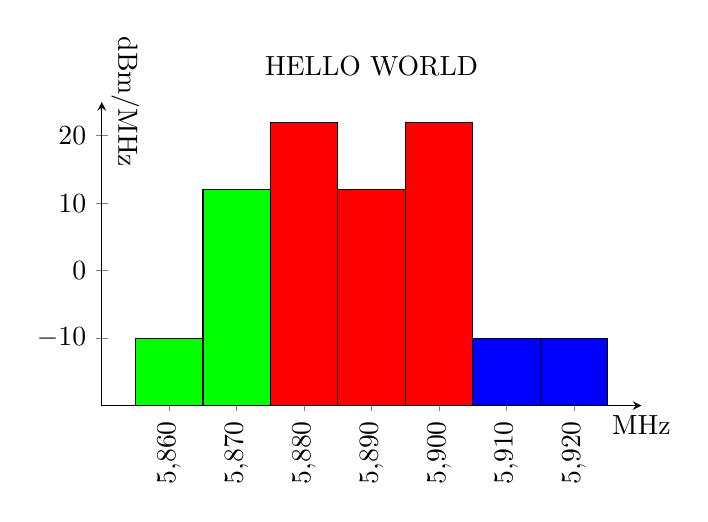
\begin{tikzpicture}
    \centering
    \begin{axis}[
        title=HELLO WORLD,
        xlabel=MHz,
        x label style={at={(axis description cs:1,0)},anchor=north},
        ylabel={dBm/MHz}, %TODO properly
        y label style={
            at={(axis description cs:0,1)},
            anchor=south,
            rotate=180
        },
        xmin=5850, xmax=5930,
        ymin=-20, ymax=25,
        x tick label style={rotate=90},
        xtick={5860, 5870, 5880, 5890, 5900, 5910, 5920},
        ytick={-10, 0, 10, 20},
        axis x line=bottom, axis y line=left,
        axis equal image
        % axis line thick
    ]
    \draw [fill=green]  (axis cs:5855,-20) rectangle (axis cs:5865,-10); %SCH4
    \draw [fill=green]  (axis cs:5865,-20) rectangle (axis cs:5875, 12); %SCH3
    \draw [fill=red]    (axis cs:5875,-20) rectangle (axis cs:5885, 22); %SCH1
    \draw [fill=red]    (axis cs:5885,-20) rectangle (axis cs:5895, 12); %SCH2
    \draw [fill=red]    (axis cs:5895,-20) rectangle (axis cs:5905, 22); %CCH
    \draw [fill=blue]   (axis cs:5905,-20) rectangle (axis cs:5915,-10); %SCH5
    \draw [fill=blue]   (axis cs:5915,-20) rectangle (axis cs:5925,-10); %SCH6
    
    \end{axis}
\end{tikzpicture}


% ITS-G5 A
    % ITS road safety related applications
    % 30 MHz
% ITS-G5 B
    % ITS non-safety application
    % 20 MHz
% ITS-G5 C
    % operations also referred to
    % broadband radio access networks (BRAN),
    % radio local area network (RLAN)
    % and wireless local area network (WLAN)

% ITS-G5 D
    % future ITS applications
    % 

% applies OFDM

% ----- explain higher OSI layers

\begin{figure}[H]
    \centering
    \includegraphics[
        width=\textwidth
    ]{ITS-G5.pdf}
    \caption{meaningful Caption about ITS-G5}
    \label{fig:iso-its-g5}
\end{figure}

% compare EU spectrum with US, (possibly) mention briefly incomparability with Japan


% Message Dictionary / OSI FACILITY layer
% EN 302 637-2 (CAM)
% EN 302 637-3 (DENM)

% mention example application (OSI application)

\subsection{Cellular-V2X (C-V2X)}
% V2X via LTE (or, future: 5G)

% ETSI TS 122 185
% US ????
                    
% https://ec.europa.eu/transport/sites/transport/files/themes/its/doc/c-its-platform-final-report-january-2016.pdf
% TS 122 185 (maybe more)



% Interoperability
% The ITS-G5 technology and the application software stack have been standardised in the European standardisation body ETSI since 2009 under a European standardisation mandate.14 Its standards are openly accessible to assure interoperability
% https://itsg5-ready-to-roll.eu/ITS-G5-FactSheet.pdf

\newpage

\section{V2X Message Sets}
% [TODO] General info, introduction to Message sets


\subsection{Cooperative Awareness Messages (CAM)}
%   ETSI EN 302 637-2

% --- explain cam structure (it's containers and each field)
% use cases, in which applications there used
% generation time

% CAM table

CAM generation frequency: 100 - 1000 ms (or 1-10Hz)
CAM data volume:
    
    Base container
    + HF Container 
    + LF Container
    = ~200 bits
    
    ITS PDU header
    + Signature
    = ~750 bits
    
    certificate = ~1 Kbit

% General structure of a CAM

% ---- [insert example CAM]
\begin{figure}[H]
    \centering
    \includegraphics[
        width=\textwidth
    ]{CAM.pdf}
    \caption{Meaningful Caption CAM}
    \label{fig:cam-structure}
\end{figure}


\subsection{Decentralized Environmental Notification Messages (DENM)}
%   ETSI EN 302 637-3

% explain DENM structure....
% its containers
%   each field

% DENM Table
\begin{figure}[H]
    \centering
    \includegraphics[
        width=\textwidth
    ]{DENM.pdf}
    \caption{meaningful caption DENM}
    \label{fig:denm-structure}
\end{figure}
